\documentclass{article}
\usepackage{array}% http://ctan.org/pkg/array
\usepackage{graphicx} % the demo option is just for the example
\usepackage{amssymb}
\usepackage{tikz}
\usepackage{xcolor}
\usepackage{fullpage}
\usepackage{xifthen}
\usepackage{setspace}
\usepackage{xstring}
\usepackage{comment}
\usepackage{svg}
\usetikzlibrary{circuits.logic.US,circuits.logic.IEC,fit}

\newcommand\addvmargin[1]{
  \node[fit=(current bounding box),inner ysep=#1,inner xsep=0]{};
}

\def\arraystretch{1.5}%  1 is the default, change whatever you need

% set font encoding for PDFLaTeX, XeLaTeX, or LuaTeX
\usepackage{ifxetex,ifluatex}
\if\ifxetex T\else\ifluatex T\else F\fi\fi T%
  \usepackage{fontspec}
\else
  \usepackage[T1]{fontenc}
  \usepackage[utf8]{inputenc}
  \usepackage{lmodern}
\usepackage{fullpage}

\title{Activité: Départ en vacances} %les aventures ordonnées de Nono l'asticot
\author{Clément Legrand \and Arnaud Lequen \and Guillaume Mescoff}

%% Colors
\definecolor{cbeige}{HTML}{FAEBD7}
\definecolor{cpink}{HTML}{FFC0CB}
\definecolor{cblack}{HTML}{010101}
\definecolor{corange}{HTML}{D2691E}
\definecolor{cred}{HTML}{FF0921}
\definecolor{cpurple}{HTML}{9683EC}
\definecolor{cyellow}{HTML}{FEF86C}
\definecolor{clightgreen}{HTML}{BEF574}
\definecolor{cdarkgreen}{HTML}{82C46C}
\definecolor{cskyblue}{HTML}{E0FFFF}
\definecolor{cgrey}{HTML}{8A8A8A}

% Couleurs utilisées dans l'exemple du disque
\definecolor{cmarron}{HTML}{AE8964}
\definecolor{cfuschia}{HTML}{ff1493}
\definecolor{climegreen}{HTML}{00ff00}
\definecolor{ccrememarron}{HTML}{cd853f}
\definecolor{clavender}{HTML}{da70d6}
\definecolor{clightgrey}{HTML}{f0f8ff}
\definecolor{cbordeau}{HTML}{a52a2a}
\definecolor{csuperblue}{HTML}{7fffd4}
\definecolor{cbrun}{HTML}{d2691e}
\definecolor{cocean}{HTML}{00ced1}
\definecolor{ckaki}{HTML}{556b2f}
\definecolor{cpika}{HTML}{ffd700}
\definecolor{clouche}{HTML}{696969}




%% Macros
% 
\newcommand{\coloritem}[2]{\IfSubStr{|cbeige|cpink|cmarron|cblack|corange|cred|cpurple|cyellow|clightgreen|cdarkgreen|cskyblue|cgrey|cfuschia|climegreen|ccrememarron|clavender|clightgrey|cbordeau|csuperblue|cbrun|cocean|ckaki|cpika|clouche|}{#1}
{\draw[black,fill=#1] (#2) circle (.25);}
{\draw (#2) node (.25) {#1};\draw[black] (#2) circle (.25);}}

% Circles
\newcommand\ccircle[1]{
\begin{tikzpicture}
  \draw[black,fill=#1] (0,0) circle (.25);
\end{tikzpicture}
}

% Tasks
\newcommand\twotaskscircles[2]{
\begin{tikzpicture}

  \coloritem{#1}{0,0}
  \draw[] (.8,0) node[]{$+$};
  \coloritem{#2}{1.6,0}
  \draw[] (2.4,0) node[]{$=$};

\end{tikzpicture}
}




\newcommand\threetaskscircles[3]{
\begin{tikzpicture}

  \coloritem{#1}{0,0}
  \draw[] (.8,0) node[]{$+$};
  \coloritem{#2}{1.6,0}
  \draw[] (2.4,0) node[]{$+$};
  \coloritem{#3}{3.2,0}
  \draw[] (4,0) node[]{$=$};
  
  \draw[] (4.5,0) to (4.5,3)  ;
  

\end{tikzpicture}
}




\newcommand\fourtaskscircles[4]{
\begin{tikzpicture}

  \coloritem{#1}{0,0}
  \draw[] (.8,0) node[]{$+$};
  \coloritem{#2}{1.6,0}
  \draw[] (2.4,0) node[]{$+$};
  \coloritem{#3}{3.2,0}
  \draw[] (4,0) node[]{$+$};
  \coloritem{#4}{4.8,0}
  \draw[] (5.6,0) node[]{$=$};

\end{tikzpicture}
}

\newcommand\taskname[1]{
\begin{tikzpicture}
\draw node[above,minimum size=2ex]{\texttt{#1}};
\end{tikzpicture}
}

\newcommand\twotask[3]{
\scalebox{1.4}{
\parbox{5cm}{
\setlength{\extrarowheight}{5pt}%
\begin{tabular}{|c|c|c|}
\hline
 \taskname{#1} & \twotaskscircles{#2}{#3} & \ccircle{white}\\
\hline
\end{tabular} \vspace{1ex}
}
}}

\begin{comment}


\newcommand\threetask[4]{
\scalebox{1.4}{
\parbox{5cm}{
\setlength{\extrarowheight}{5pt}%
\begin{tabular}{|c|c|c|}
\hline
 \taskname{#1} & \threetaskscircles{#2}{#3}{#4} & \ccircle{white}\\
\hline
\end{tabular} 
}
}}

\end{comment}









\newcommand\fourtask[5]{
\scalebox{1.4}{
\parbox{5cm}{
%


 
 \begin{tikzpicture}
 %\draw node[above,minimum size=2ex]{\texttt{#1}};
 \draw (-1.8,0)  rectangle (10.5,0.8);
 \draw (-0.5,0.1)  rectangle (4,0.7);
 \draw (2.75,0.05)  rectangle (7.5,0.75);
 
 \draw [-] (6.5,0.05) to (6.5,0.75);
 
 \draw [-] (9.5,0) to (9.5,0.8);
 
 
 \draw[] (8.0,0.4) node[]{$+$};
 \coloritem{#5}{8.7,0.4}
 
 \draw[black,fill=white] (10,0.4) circle (.25);
 
 \coloritem{#2}{0,0.4}
  \draw[] (.8,0.4) node[]{$+$};
  \coloritem{#3}{1.6,0.4}
  \draw[] (2.4,0.4) node[]{$=$};
  
  \draw[] (2.75,0.1) to (2.75,0.7) ;
  
  \draw[black,fill=white] (3.2,0.4) circle (.25);
  
  \draw[] (4.4,0.4) node[]{$+$};
  \coloritem{#4}{5.2,0.4}
  \draw[] (6,0.4) node[]{$=$};
  \draw[black,fill=white] (7,0.4) circle (.25);
  
  \draw [-] (-0.9,0) to (-0.9,0.8);
  
  
  
  \draw (-1.3,.45) node {#1};
  
  
  
  
  
   \, \, \, \,\, \,\, \,\, \,\, \,\, \,\, \,\, \,\, \,\, \,\, \,
 %\draw[black,fill=#2] (0,0.4) circle (.25);
 
 


\end{tikzpicture}  
}}\vspace{2mm}}








\newcommand\threetask[4]{
\scalebox{1.4}{
\parbox{5cm}{
%


 
 \begin{tikzpicture}
 %\draw node[above,minimum size=2ex]{\texttt{#1}};
 \draw (-1.8,0)  rectangle (7.5,0.8);
 \draw (-0.5,0.1)  rectangle (4,0.7);
 
 
 
 \coloritem{#2}{0,0.4}
  \draw[] (.8,0.4) node[]{$+$};
  \coloritem{#3}{1.6,0.4}
  \draw[] (2.4,0.4) node[]{$=$};
  
  \draw[] (2.75,0.1) to (2.75,0.7) ;
  
  \draw[black,fill=white] (3.2,0.4) circle (.25);
  
  \draw[] (4.4,0.4) node[]{$+$};
  \coloritem{#4}{5.2,0.4}
  \draw[] (6,0.4) node[]{$=$};
  \draw[black,fill=white] (7,0.4) circle (.25);
  
  \draw [-] (-0.9,0) to (-0.9,0.8);
  
  \draw [-] (6.5,0) to (6.5,0.8);
  
  \draw (-1.3,.45) node {#1};
  
  
  
  
  
   \, \, \, \,\, \,\, \,\, \,\, \,\, \,\, \,\, \,\, \,\, \,\, \,
 %\draw[black,fill=#2] (0,0.4) circle (.25);
 
 \vspace{1ex}
 

\end{tikzpicture} 
}
} \vspace{2mm}
}



\begin{document}
\maketitle
\begin{center}
  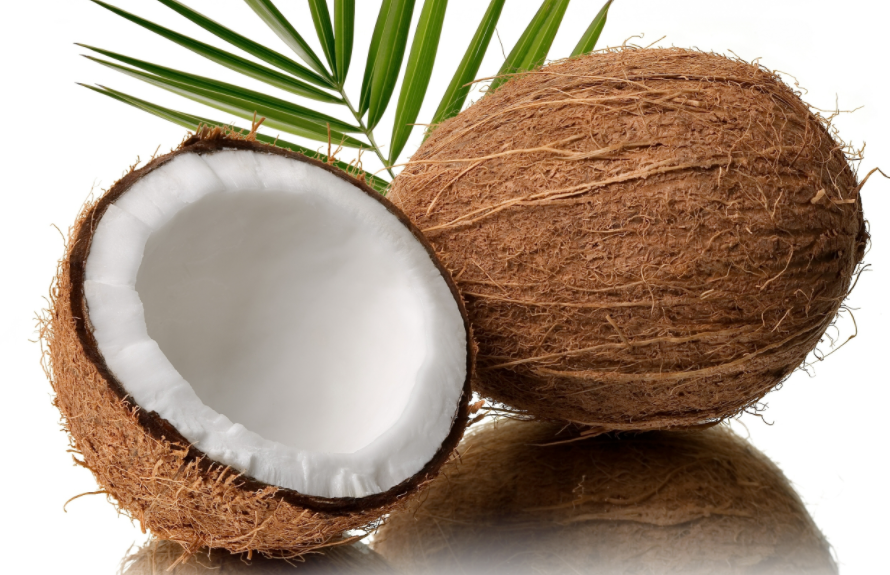
\includegraphics[width=0.2\textwidth]{assets/coco.png}  
\end{center}




\section{Présentation de l'activité}

16h30. La cloche sonne la fin de l'école et le début des vacances. Mais avant de partir à la plage, il reste une chose à faire: préparer les affaires. Vite, maman doit mettre toutes les valises dans la voiture. Mais avant cela, il faudrait déjà que papa ait bien fermé toutes les valises. Et les enfants doivent, encore avant, préparer les bouées et leurs maillots de bain. Il faut, en parallèle, avoir coupé l'électricité à la maison, mais pas avant d'avoir préparé les paninis et d'avoir regonflé les pneus.

Une famille mal organisée perdrait énormément de temps, avec les parents qui doivent attendre que les enfants aient fini leurs valises pour continuer à charger la voiture, ou avec le père qui finit par charger seul la voiture pendant que les autres attendent, toutes les tâches ayant été effectuées par ailleurs. Mais, avec une bonne planification, toute la famille peut partir en vacances en un temps record.

Au cours de cette activité, nous aborderont donc le problème de l'ordonnancement, présent dans la vie de tous les jours, mais non moins crucial dans bien d'autres domaines scientifiques et techniques. En effet, il est non seulement présent sur les plans techniques et théoriques de l'informatique, mais aussi dans bien d'autres domaines: production industrielle, aérospatial, logistique...

De manière plus générale, le problème d'ordonnancement cherche à trouver une manière d'accomplir un ensemble de tâches dépendantes les unes des autres, en parallèle, et ce le plus rapidement possible. Dans cette activité, les élèves vont devoir traiter de manière la plus efficace possible une liste de tâches données. Selon les caractéristiques de l'instance traitée, l'algorithme présenté peut être différent.


    
\section{Description de l'activité}
Au début de l'activité les participants sont invités à former des groupes d'au moins 3 personnes, et d'au plus 5 personnes. 

Chaque groupe reçoit alors, selon le problème, un ensemble de tâches à effectuer de la manière la plus rapide possible. (Il pourrait même être possible de chronométrer les différents groupes, pour ajouter un aspect compétitif à l'activité, principalement au début lors de la découverte du problème. Cela permet de voir quels idées intuitives sont proposées par les groupes pour effectuer les tâches le plus vite possible, avant de leur proposer des algorithmes basiques dans la suite).

Pour effectuer les tâches, chaque élève de chaque groupe aura à sa disposition un disque de déchiffrement qui sont tous identiques et restent inchangés au cours de l'activité (voir la prochaine section pour une explication plus détaillée du fonctionnement des disques).

Une fois qu'un groupe a terminé sa liste de tâches, en attendant que les autres groupes terminent, il est invité à réfléchir à une manière d'organiser la réalisation des tâches, pour gagner du temps par rapport à ce qui a été fait. Une fois l'activité introductive passée, il peut être conseillé (selon le bon vouloir de l'organisateur) pour chaque groupe, de d'abord écrire l'ordre des tâches à faire et de les répartir aux autres membres du groupe.

Une fois que la plupart des groupes ont terminé l'activité, une mise en commun est réalisée. 
Les particularités des tâches sont expliquées, les problèmes rencontrés par les groupes sont mis en commun, et une réflexion autour de l'algorithme à utiliser est lancée, ou bien directement proposée par l'organisateur.  

\section{Description du matériel}

\subsection{Les tâches}

%Papier de tâches

%De petits morceaux de papiers qui constituent une tâche à effectuer par une ligne de production (=un élève). Toutes les tâches ont un identifiant. Elles demandent de combiner deux couleurs, et quelquefois, on ne spécifie pas la couleur sur la tâche, mais l'identifiant d'une autre tâche. Il faut alors substituer l'identifiant par la couleur finalement obtenue après avoir terminé l'autre tâche. Cela crée un réseau de dépendances, qui est une contrainte au coeur du problème.

Chaque tâche à effectuer est représentée sur un bout de papier, dont le dernier rond est à colorier par l'élève, de cette forme:

\subsubsection{Tâches simples}
\begin{center}
    \twotask{T}{clouche}{cpika}
\end{center}
Les tâches simples ne dépendent d'aucune autre tâche. Elles contiennent une somme de deux couleurs au moins, le résultat de la tâche s'obtient alors grâce au déchiffreur. Sur cet exemple, l'élève doit combiner la couleur gris foncé et la couleur jaune afin d'obtenir la couleur associée à la tâche \textsf{T}.

Chaque tâche à effectuer est représentée sur un bout de papier, dont le dernier rond est à colorier par l'élève, de cette forme:


\subsubsection{Tâches complexes}
\begin{center}
    \twotask{S}{T}{ckaki}
\end{center}

Les tâches complexes dépendent d'au moins une autre tâche. On les repère car elles ont le nom d'une autre tâche dans leur somme. Il faut alors d'abord effectuer la tâche inscrite dans le cercle, et remplacer le nom de la tâche par la couleur obtenue. 


\subsection{Les disques}

%Disques de composition

%Permettent de combine les couleurs sur les tâches, pour accomplir ces tâches. A une forme analogue à un disque de César, et un fonctionnement analogue à un monoïde.


Chaque groupe d'élèves dispose de plusieurs disques, désignés dans la suite par le terme déchiffreur, qui vont leur servir à effectuer les tâches. 

Un déchiffreur consiste en deux cercles concentriques superposés. Le cercle intérieur peut tourner par rapport au cercle extérieur. Sur chaque cercle, 12 couleurs sont disposées. Des flèches sont présentes sur le cercle intérieur et passent par une seule couleur $c_{int}$. Si la base de la flèche relie une couleur $c_{ext}$ à une couleur $c_{res}$ à la pointe de la flèche, on peut écrire le résultat suivant: $c_{ext} + c_{int} = c_{res}$. 

\begin{center}
    \includesvg[width=0.5\textwidth]{assets/disque_complet.svg}
\end{center}

Par exemple, si on souhaite réaliser une tâche $\textsf{T}$ précédente, il faut aligner les deux disques de sorte à ce que la couleur gris foncé soit sur le disque extérieur, et la couleur jaune soit sur le disque intérieur. On suit ensuite la flèche partant du rond gris, et on tombe sur la couleur bleu foncé. On remplit alors la couleur de la tâche.



A remarquer que la couleur à gauche du signe plus (+) doit être sur le disque extérieur, et l'autre sur le disque intérieur. En effet, avec l'exemple précédent, en mettant la couleur jaune sur le disque extérieur et la couleur gris foncé sur le disque intérieur, on tombe sur la couleur marron, ce qui n'est pas correct. 


\begin{center}
\scalebox{1.4}{
\parbox{5cm}{
\setlength{\extrarowheight}{5pt}%
\begin{tabular}{|c|c|c|}
\hline
 \taskname{T} & \twotaskscircles{clouche}{cpika} & \ccircle{cocean}\\
\hline
\end{tabular} \vspace{1ex}
}
}
\end{center}

Une fois la couleur de la tache $\textsf{T}$ déterminée, on peut trouver la couleur de la tâche S. Il suffit pour cela de faire tourner le disque d'un cran dans le sens des aiguilles d'une montre, pour aligner la couleur bleu foncé et la couleur kaki. On suit alors la flèche de la couleur kaki, et on obtient bleu ciel.

\begin{center}
\scalebox{1.4}{
\parbox{5cm}{
\setlength{\extrarowheight}{5pt}%
\begin{tabular}{|c|c|c|}
\hline
 \taskname{S} & \twotaskscircles{T}{ckaki} & \ccircle{csuperblue}\\
\hline
\end{tabular} \vspace{1ex}
}
}
\end{center}



\section{Déroulement des activités}

Chaque groupe dispose d'un ensemble de tâches à effectuer, et le travail est terminé lorsque le groupe a retrouvé les couleurs de chaque tâche. Chaque élève représente une ligne de production qui peut travailler en parallèle des autres élèves, et de manière a priori indépendante. A terme les élèves doivent se coordonner afin de mutualiser au mieux les efforts de résolution des tâches et de répartir le travail du mieux possible.

\subsection{Problème 1 - Découverte et prise en main du matériel}

\begin{itemize}
    \item \textbf{Objectif}: Prendre en main le matériel de base, qui permet d'effectuer les tâches.
    \item \textbf{Matériel}: Un disque par élève, un ensemble de tâches (l'ensemble du problème 1)
    \item \textbf{Consigne}: Résoudre le problème le plus rapidement possible
\end{itemize}

On s'attend à ce que les élèves n'aient pas de stratégie particulière de résolution, et essaient de résoudre les tâches en les choisissant de manière aléatoire, et en les remettant dans le tas de tâches jusqu'à ce qu'ils arrivent à trouver une tâche réalisable (i.e., sans dépendance non déjà calculée), et le but est de leur faire découvrir qu'ils perdent beaucoup de temps à remonter les dépendances de chaque tâche.

\subsection{Problème 2 - Premières abstractions et heuristiques gloutonnes}

\begin{itemize}
    \item \textbf{Objectif}: Introduire une première manière d'abstraire l'espace de recherche de solution, afin de prendre du recul sur l'exploration, en ayant une stratégie de résolution pré-établie. 
    \item \textbf{Matériel}: Un disque par élève, un ensemble de tâches par groupe (l'ensemble 2)
    \item \textbf{Consigne}: Trouver un ordre d'exécution des tâches, en faisant attention à les répartir du mieux possible sur l'ensemble des élèves, afin de résoudre le problème le plus rapidement possible.
\end{itemize}

L'idée est d'introduire un diagramme de Gantt pour représenter les différents élèves, et de représenter les tâches, plus ou moins longues, par des rectangles plus ou moins longs. Cela permet de savoir à l'avance quelles tâches et dans quel ordre chaque élève va devoir effectuer, et donc de non seulement perdre moins de temps en cherchant quelle tâche peut être effectuée, mais aussi de ne pas interférer négativement avec les autres élèves. En effet, avec une planification correcte, les élèves peuvent anticiper les dépendances entre tâches, même si ce point est encore peu développé à ce stade.

Un des principaux intérêts de cette partie est de présenter des ensembles de tâches aux dépendances faibles, mais avec des tâches de grandes durées. En répartissant correctement les tâches, on évite les situations où un élève doit finir une tâche très longue seul, alors que les autres vont devoir l'attendre car toutes les autres sont terminées.

Un algorithme glouton permet d'éviter ce genre d'aléas assez facilement, et a le mérite d'être simple à aborder, tout en étant une technique souvent utilisée en informatique.

On peut éventuellement donner aux élèves une assignation des tâches sur le diagramme de Gantt choisie par l'encadrant, pour commencer.

\subsection{Problème 3 - Espace de recherche et dépendances}

\begin{itemize}
    \item \textbf{Objectif}: Abstraire les dépendances entre tâches dans l'espace de recherche des solutions. Cela permet d'introduire, en outre, la notion de graphe dirigé, et une sémantique associée.
    \item \textbf{Matériel}: Un disque par élève, un ensemble de tâches par groupe (l'ensemble 3)
    \item \textbf{Consigne}: Trouver un ordre d'exécution des tâches, en faisant attention à bien prendre en compte les dépendances entre elles afin de ne pas avoir à revenir en arrière.
\end{itemize}

En utilisant la méthode PERT, qui vise à représenter les dépendances entre tâches par un graphe, on dessine le graphe de dépendances et on identifie le chemin critique. On a alors un ordre partiel, qui dicte la manière dont les tâches doivent être effectuées.

%Montrer un graphe de dépendances (graphe causal). Méthode du chemin critique (PERT)

%Notes en vrac :

%Algorithmes à présenter:

%Shortest job first, shortest remaining time?

%Longest job first

%Méthode PERT

%Ordonnancement en ligne ?

%Round Robin

%Peut-être ne pas utiliser des disques de César, mais des planches de symboles découpées en cases numérotées. Les cases numérotées ont toutes un type de symboles dominant, et il donne la couleur de l'identifiant associé

\section{C'est de l'informatique parce que...}
A la fin de l'activité (au cours des 10 dernières minutes par exemple), on présente pourquoi cette activité est en fait de l'informatique.
\begin{itemize}
    \item On présente un problème qui est crucial pour un grand nombre de systèmes informatiques (OS avec la répartition des \textit{jobs}, systèmes distribués...), mais aussi pour de nombreux systèmes industriels (gestion de lignes de production, ordonnancement de constellations de satellites...)
    \item C'est un problème combinatoire qui comporte un grand nombre de candidats de solutions, et dont l'ensemble de solutions possibles est tellement grand et complexe que même un ordinateur ne peut pas énumérer tous les candidats possibles. Il faut donc que l'ordinateur même trouve des astuces de calcul.
\end{itemize}


\end{document}